\documentclass{article}
\usepackage{geometry}
\usepackage{amsmath}
\usepackage{amsfonts}
\usepackage{amssymb}
\usepackage{amsthm}
\usepackage{parskip}
\usepackage{multicol}
\usepackage{xcolor}
\usepackage{fancyhdr}
\usepackage{physics}
\usepackage{graphicx} % Required for inserting images
\usepackage{hyperref}
\usepackage{enumitem}
\usepackage{mathtools}
\usepackage[utf8]{inputenc}
\usepackage[T1]{fontenc}
\usepackage{centernot}

% commands
\newcommand{\deq}{\vcentcolon=}
\newcommand{\idd}{\text{đ}}
\newcommand{\nimplies}{\centernot\implies}
\newcommand{\vc}[1]{\boldsymbol{#1}}

% margin settings
\geometry{
    a4paper,
    left=7mm,
    right=7mm,
    top=2cm,
    bottom=7mm
}

% testing
\usepackage{blindtext}

% proof environments
\newtheorem{definition}{Definition}[section]
\newtheorem{theorem}{Theorem}[section]
\newtheorem{corollary}{Corollary}[theorem]
\newtheorem{lemma}[theorem]{Lemma}
\newtheorem*{remark}{Remark} % unnumbered remarks

% header and footer
\pagestyle{fancy}
\fancyfoot{} % removes footer
\fancyhf{}
\renewcommand{\headrulewidth}{0.5pt}
\fancyhead[L]{Honours algebra}
\fancyhead[R]{\thepage}

\begin{document}

\begin{multicols*}{3}
\noindent

\subsubsection*{D: Functions}
A function $f:X\rightarrow Y$ is an assignment
of an element of $Y$ to \underline{each} element of $X$.
\begin{enumerate}
    \item $f$ is \textbf{injective} if:
    \begin{align*}
        &\forall x_1,x_2\in X;
        f(x_1)=f(x_2) \\ &\implies x_1=x_2
    \end{align*}
    and this implies $|X|\leq|Y|$.

    \item $f$ is \textbf{surjective} if:
    $$\forall y\in Y;\exists x\in X: y=f(x)$$
    and this implies $|X|\geq|Y|$.

    \item $f$ is \textbf{bijective}
    if it is injective and surjective.
\end{enumerate}
\begin{center}
    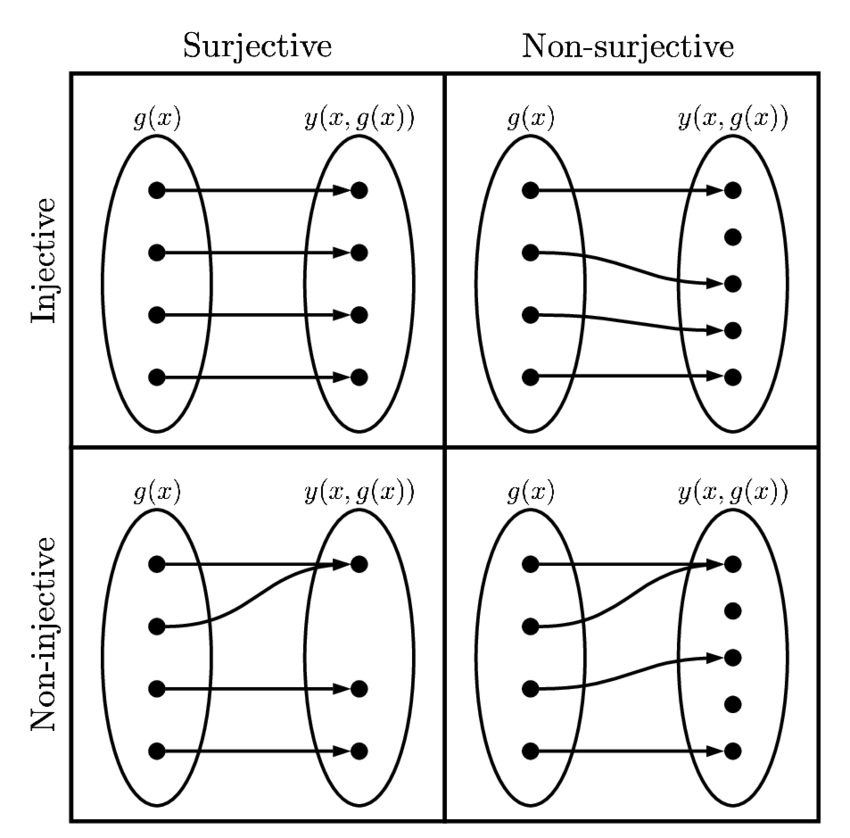
\includegraphics[scale=0.2]{f00.png}
\end{center}

\subsubsection*{D: Groups}
A group $G$ is a set with a composition
operator $(\circ)$ such that $\forall x,y,z,\in G$:
\begin{enumerate}
    \item $x\circ y=xy$
    
    \item $(xy)z=x(yz)$
    
    \item $\exists e\in G: ex=xe=x$
    
    \item $\exists x^{-1}\in G: xx^{-1}=x^{-1}x=e$
\end{enumerate}
$G$ is \textbf{Abelian} if 
$\forall x,y\in G; xy=yx$.

\subsubsection*{D1.2.1(i): Fields}
A field $F$ is a set defined with addition
and multiplication such that:
\begin{enumerate}
    \item $(+):F\times F\rightarrow F;
    (\lambda,\mu)\mapsto\lambda+\mu$

    \item $(\cdot):F\times F\rightarrow F;
    (\lambda,\mu)\mapsto\lambda\cdot\mu$

    \item $\exists (-\lambda)\in F:
    \lambda+(-\lambda)=0_F$

    \item $\exists (\lambda^{-1})\in F:
    \lambda\cdot(\lambda^{-1})=1_F$ \\
    except when $\lambda=0$.

    \item $(+)$ and $(\cdot)$
    are associative, \\ commutative
    and distributive.
\end{enumerate}

\subsubsection*{Remark}
$(F,+)$ and $(F\hspace{0.02in}\backslash
\hspace{0.02in}\{0_F\},\cdot)$ are groups.

\subsubsection*{Remark}
Let $n$ be prime or a prime power.
Then $\mathbb{F}_n$ is a finite field with $n$ elements
under modulo $n$.
Also, $\mathbb{Q}$ and $\mathbb{R}$ are fields.

\subsubsection*{D1.2.1(ii): Vector spaces}
A vector space $V$ over a field $F$ is an Abelian group $V\deq(V,+)$
with mapping:
$$F\times V\rightarrow V;
(\lambda,\vc{v})\mapsto
\lambda\vc{v}$$
where for $\forall\lambda, \mu\in F$ and
$\forall\vc{v},\vc{w}\in V$:
\begin{enumerate}
    \item
    $\lambda(\vc{v}+\vc{w})
    =(\lambda\vc{v})+(\mu\vc{w})$

    \item $(\lambda+\mu)\vc{v}
    =(\lambda\vc{v})+(\mu\vc{w})$

    \item $\lambda(\mu\vc{v})=(\lambda\mu)\vc{v}$
    
    \item $1_F\vc{v}=\vc{v}$
\end{enumerate}
and is known as a \textcolor{red}{$F$-vector space}.

\subsubsection*{Remark}
Let $V$ be a $F$-vector space and $\vc{v}\in V$.
\begin{enumerate}
    \item $0\vc{v}=0$
    \item $(-1)\vc{v}=-\vc{v}$
    \item $\lambda\vc{0}=\vc{0}$
    for $\forall\lambda\in F$.
\end{enumerate}

\subsubsection*{D: Cartesian products}
The \textbf{cross product} of sets $X_1,\dots,X_n$ is:
$$X_1\times\cdots\times X_n
\deq\{(x_1,\dots,x_n):x_i\in X_i\}$$
with bijection $X^n\times X^m\rightarrow X^{n+m}$.

The \textbf{projection} of a cross product is:
\begin{align*}
    \text{pr}_i &:X_1\times\cdots\times X_n
    \rightarrow X_i; \\
    &(x_1,\dots,x_n)\mapsto x_i.
\end{align*}

\subsubsection*{D1.4.1: Vector subspaces}
A vector subspace $U$ of $F$-vector space $V$
has the following properties:
\begin{enumerate}
    \item $U\subset V$ and $\vc{0}\in U$.
    \item Let $\vc{u},\vc{v}\in U$
    and $\lambda\in F$. \\ Then
    $\vc{u}+\vc{v}\in U$ and $\lambda\vc{u}\in U$.
\end{enumerate}
and is also a vector space.

\subsubsection*{P1.4.5}
Let $T\subset V$ where $V$ is a $F$-vector space.
Then for all vector subspaces containing $T$,
there exists a \underline{smallest} vector subspace:
$$\text{span}(T)=\langle T\rangle_F\subset V$$
known as the vector subspace generated by $T$,
or the span of $T$.

\subsubsection*{D1.4.7: Generating set}
Let $T\subset V$ where $V$ is a $F$-vector space.
Set $T$ is a \textbf{generating set} of $V$ if:
$$\text{span}(T)=V$$
and is the linear combination of vectors in $T$
over field $F$. $V$ is \textbf{finitely generated}
if its generating set $T$ is finite.

\subsubsection*{D1.4.9: Power sets}
The power set of set $X$ is:
$$\mathcal{P}(X)\deq\{U:U\subseteq X\}.$$
Let $\mathcal{U}\subseteq\mathcal{P}(X)$. Then:
$$\bigcup_{U\in\mathcal{U}}U
\deq\{x\in X:(\exists U\in\mathcal{U}:x\in U)\}$$
$$\bigcap_{U\in\mathcal{U}}U
\deq\{x\in X:\forall U\in\mathcal{U};x\in U\}.$$

\subsubsection*{D1.5.1: Linear independence}
Let $V$ be a $F$-vector space and $L\subseteq V$. \\
Subset $L$ is \textbf{linearly independent} if:
\begin{align*}
    &\alpha_1\vc{v}_1+\dots+\alpha_r\vc{v}_r=\vc{0} \\
    &\implies \alpha_1=\dots=\alpha_r=0
\end{align*}
for $\vc{v}_i\in L$
and is pairwise distinct.

\subsubsection*{Remark}
$L$ is linearly dependent if some $\alpha_i\neq0$.

\subsubsection*{D1.5.8: Basis}
A basis of a vector space $V$ is a \textbf{linearly independent}
\underline{generating set} in $V$.

\subsubsection*{T1.5.11}
Let $V$ be a $F$-vector space.

Then $A=\{\vc{v}_1,\dots,\vc{v}_r\}$ is a basis of $V$
\textbf{if{}f} the following \textcolor{red}{evaluation mapping}:
$$\Phi:F^r\rightarrow V;$$
$$(\alpha_1,\dots,\alpha_r)\mapsto
\alpha_1\vc{v}_1+\dots+\alpha_r\vc{v}_r$$
is a bijection.

\subsubsection*{Remark}
$\Phi$ is surjective if $A$ is generating.

\subsubsection*{T1.5.12}
Let $V$ be a vector space and $E\subseteq V$.
Then the following statements are equivalent:
\begin{enumerate}
    \item $E$ is a basis of $V$.
    
    \item $E$ is minimal among all generating sets,
    or that $E\hspace{0.02in}\backslash\hspace{0.02in}
    \{\vc{e}\}$ is not a basis for $\forall\vc{e}\in E$.

    \item $E$ is maximal amongst all linearly independent subsets.
    i.e. $E\hspace{0.01in}\cup\hspace{0.01in}\{\vc{v}\}$
    is linearly dependent for $\forall\vc{v}\in V$.
\end{enumerate}

\subsubsection*{C1.5.13}
Every finitely generated vector space has a finite basis.

\subsubsection*{T1.5.14}
Let $V$ be a vector space.
\begin{enumerate}
    \item Let $L\subseteq V$ be linearly independent and
    set $E$ be minimal amongst all generating sets of $V$.
    Let $L\subseteq E$.
    Then $E$ is a basis of $V$.

    \item Let $E\subseteq V$ be a generating set and
    $L$ be maximal amongst all linearly independent
    subsets of $V$. 
    
    Let $L\subseteq E$. Then $E$ is a basis of $V$.
\end{enumerate}

\subsubsection*{D1.5.15}
Let $X$ be a set and $F$ be a field. Then:
$$\text{maps}(X,F)\deq\{f:(\forall f:X\rightarrow F)\}$$
and is a $F$-vector space under pointwise addition and
multiplication via scalars.

Let $F\langle X\rangle\subseteq\text{maps}(X,F)$ be
the subset of all mappings that sends all but finitely many
elements of $X$ to $0$:
$$F\langle X\rangle\deq
\left\{f:\bigl(\forall f:X\rightarrow\{0\}\bigr)\right\}.$$
It contains all linear combinations of $X$
in $F$ and forms a vector subspace.

\subsubsection*{T1.5.16}
Let $V$ be a $F$-vector space.

Then $(\vc{v}_i)_{i\in I}$ is a basis for $V$ \textbf{if{}f}:
\begin{align*}
    \forall\vc{v}\in V;\exists!(a_i)_{i\in I}\subseteq F:
    \vc{v}=\sum_{i\in I}a_i\vc{v}_i.
\end{align*}

\subsubsection*{T1.6.1}
Let $V$ be a vector space.
Let $L\subset V$ be a linearly independent subset
and $E\subseteq V$ a generating set.
Then $|L|\leq|E|$.

\subsubsection*{T1.6.2: Steinitz exchange theorem}
Let $V$ be a vector space, $L\subset V$ be a finite
linearly independent subset and $E\subseteq V$
be a generating set.

Then there exists an \textbf{injective} function
$\phi:L\rightarrow E$ such that:
$$\bigl(E\hspace{0.02in}\backslash\hspace{0.02in}
\phi(L)\bigr)\cup L
\hspace{0.05in}\text{is a generating set for $V$.}$$

\subsubsection*{L1.6.3: Exchange lemma}
Let $V$ be a vector space. Let $M\subset V$ be a finite
linearly independent subset and $E\subseteq V$
be a generating set where $M\subseteq E$.

If $\exists\vc{w}\in V\hspace{0.02in}\backslash\hspace{0.02in} M$
such that set $M\cup\{\vc{w}\}$ is linearly independent then:
$$\exists\vc{e}\in E\hspace{0.02in}\backslash\hspace{0.02in} M:
\bigl(E\hspace{0.02in}\backslash\hspace{0.02in}
\vc{e}\bigr)\cup\{\vc{w}\}\hspace{0.04in}\text{is generating.}$$

\subsubsection*{C1.6.4}
Let $V$ be a finitely generated vector space.
\begin{enumerate}
    \item $V$ has finite basis.
    
    \item $V$ cannot have infinite basis.
    
    \item Any two basis of $V$ have the
    same number of elements.
\end{enumerate}

\subsubsection*{D1.6.5: Dimension}
The dimension of finite $F$-vector space $V$ is the
cardinality of one of its basis. 

For infinite vector spaces: $\dim(V)=\infty$.
We also define $\dim(\{\vc{0}\})\deq0$.

\subsubsection*{C1.6.7}
Let $V$ be a finitely generated vector space.
\begin{enumerate}
    \item Every linearly independent $L\subseteq V$
    has \textbf{at most} $\dim(V)$ elements and \\
    if $|L|=\dim(V)$ then $L$ is a basis.

    \item Every generating set $E\subseteq V$ has \\
    \textbf{at least} $\dim(V)$ elements and \\
    if $|E|=\dim(V)$ then $E$ is a basis.
\end{enumerate}

\subsubsection*{C1.6.8}
A proper vector subspace of a vector space 
with finite dimension has itself a strictly smaller dimension.

\subsubsection*{T1.6.10: Dimension theorem}
Let $V$ be a vector space and 
$U,W\subseteq V$ be vector subspaces. Then:
\begin{align*}
    &\dim(U+W)+\dim(U\cap W) \\
    &=\dim(U)+\dim(W)
\end{align*}
for $U+W\deq\langle U\hspace{0.02in}
\cup\hspace{0.02in}W\rangle\subseteq V$.

\subsubsection*{D1.7.1: Linear mappings}
Let $V$ and $W$ be $F$-vector spaces. \\
A mapping $f:V\rightarrow W$ is \textbf{$F$-linear} or a
\textbf{homomorphism} of vector spaces if for
$\forall\vc{v}_1,\vc{v}_2\in V$ and $\forall\lambda\in F$:
\begin{enumerate}
    \item $f(\vc{v}_1+\vc{v}_2)=f(\vc{v}_1)+f(\vc{v}_2)$
    \item $f(\lambda\vc{v}_1)=\lambda f(\vc{v}_1)$.
\end{enumerate}
Furthermore bijective linear mappings are an \textbf{isomorphism}
of vector spaces.

A homomorphism from a vector space to itself
is an \textbf{endomorphism}.

An isomorphism of a vector space to itself
is an \textbf{automorphism}.

\subsubsection*{D1.7.5: Fixed points}
In a linear mapping a fixed point is sent to itself.
For mapping $f:X\rightarrow X$
the \textbf{set of fixed points} is:
$$X^f=\{x\in X:f(x)=x\}.$$

\subsubsection*{D1.7.6: Complementary subspaces?}
Vector subspaces $V_1,V_2$ of vector space $V$
are \textbf{complementary} if the mapping:
$$V_1\times V_2\rightarrow V$$
is a bijection.

\subsubsection*{T1.7.7}
A $F$-vector space $V$ is isomorphic to $F^n$
\textbf{if{}f} $\dim(V)=n$,
for $n\in\mathbb{N}$ and $F$ a field.

\subsubsection*{L1.7.8}
Let $V,W$ be $F$-vector spaces and let $B$
be a basis of $V$. Then the following mapping:
\begin{align*}
    \hom_F(V,W)\rightarrow\text{maps}(B,W);
    f\mapsto f_B
\end{align*}
is a bijection.

\subsubsection*{Remark}
Let $V,W$ be $F$-vector spaces.
The set of all homomorphisms from $V$ to $W$ is:
$$\hom_F(V,W)\subseteq\text{maps}(B,W).$$

\subsubsection*{P1.7.9}
Let $f:V\rightarrow W$ be a linear mapping,
where $V,W$ are vector spaces.
\begin{enumerate}
    \item If $f$ is injective, there exists map
    $g:W\rightarrow V$ such that $g\circ f=\text{id}_V$.
    i.e. it has a \textbf{left inverse}.
    
    \item If $f$ is surjective, there exists map
    $g:W\rightarrow V$ such that $f\circ g=\text{id}_W$.
    i.e. it has a \textbf{right inverse}.
\end{enumerate}

\subsubsection*{D1.8.1: Image and kernel}
Let $f:V\rightarrow W$ be a linear mapping. \\
The \textbf{image} of this linear mapping $f$ is:
$$\text{im}(f)\deq f(V)\subseteq W$$
and is a vector subspace of $W$.

The \textbf{kernel} of this linear mapping $f$ is:
$$\ker(f)\deq f^{-1}(\vc{0})
=\{\vc{v}\in V:f(\vc{v})=\vc{0}\}$$
and is the preimage of the zero vector in
linear mapping $f$.

\subsubsection*{L1.8.2}
A linear mapping $f:V\rightarrow W$ is injective
\textbf{if{}f} $\ker(f)=\{\vc{0}\}$.

\subsubsection*{T1.8.4: Rank-nullity theorem}
Let $f:V\rightarrow W$ be a linear mapping and
$V,W$ are vector spaces. Then:
$$\dim(V)=\dim\Bigl(\ker(f)\Bigr)
+\dim\Bigl(\text{im}(f)\Bigr).$$

\subsubsection*{T2.1.1}
Let $F$ be a field and $m,n\in\mathbb{N}$.

Then there exists a bijection:
$$M:\hom_F(F^m,F^n)\rightarrow\text{mat}(n\times m;F);$$
$$f\mapsto[f]$$
and attaches each linear mapping $f$ with its
\textbf{representing matrix} $M(f)\deq[f]$.

\subsubsection*{Remark}
The set of matrices with \textcolor{red}{$n$ rows}
and \textcolor{red}{$m$ columns} with entries in field $F$ is:
$$\text{mat}(n\times m;F).$$

\subsubsection*{D2.1.6: Matrix products}
The product $A\circ B=AB$ is defined:
$$(AB)_{ik}=\sum_{j=1}^{m}A_{ij}B_{jk}$$
where $A\in\text{mat}(n\times m;F)$, $F$ a field,
$B\in\text{mat}(m\times\ell;F)$ and $m,n,\ell\in\mathbb{N}$.
This is matrix multiplication, with mapping:
\begin{align*}
    &\text{mat}(n\times m;F)\times\text{mat}(m\times\ell;F) \\
    &\rightarrow\text{mat}(n\times\ell;F);
\end{align*}
$$(A,B)\mapsto AB.$$

\subsubsection*{T2.1.8}
Let $g:F^{\ell}\rightarrow F^m$ and
$f:F^{m}\rightarrow F^{n}$ be linear mappings.
Then $[f\circ g]=[f]\circ[g]$.

\subsubsection*{P2.1.9}
Let $A,A'\in\text{mat}(n\times m;F)$. \\
Let $B,B'\in\text{mat}(m\times\ell;F)$. \\
Let $C,C'\in\text{mat}(\ell\times k;F)$. \\
Let $k,\ell,m,n\in\mathbb{N}$ and denote $I=I_m$
as the $(m\times m)$ identity matrix. Then:
\begin{enumerate}
    \item $(A+A')B=AB+A'B$
    \item $A(B+B')=AB+AB'$
    \item $IB=B$
    \item $AI=A$
    \item $(AB)C=A(BC)$.
\end{enumerate}

\subsubsection*{D2.2.1: Invertible matrices}
A matrix $A$ is \textbf{invertible} if:
$$\exists B,C:
BA=I\hspace{0.05in}\text{and}\hspace{0.05in}AC=I.$$

\subsubsection*{D2.2.2: Elementary matrices}
Elementary matrices are square matrices that differs from
the identity matrix by at most one entry.

\subsubsection*{T2.2.3}
Every square matrix with entries in a field can be written
as a \underline{product} of elementary matrices.

\subsubsection*{D2.2.4: Smith normal form}
Matrices with non-zero entries along the diagonal are
in Smith normal form. e.g:
$$\begin{pmatrix}
    1 & 0 & 0 & 0 & 0 \\
    0 & 1 & 0 & 0 & 0 \\
    0 & 0 & 1 & 0 & 0
\end{pmatrix}$$

\subsubsection*{T2.2.5}
For every $A\in\text{mat}(n\times m;F)$, \\
there exists invertible matrices $P$ and $Q$ 
such that $PAQ$ is of Smith normal form.

\subsubsection*{D2.2.7: Column and row rank}
Let matrix $A\in\text{mat}(n\times m;F)$.

The column rank of $A$ is the dimension of the subspace
of $F^n$ generated by the columns of $A$.

Similarly the row rank of $A$ is the dimension of the subspace
of $F^m$ generated by the rows of $A$.

\subsubsection*{T2.2.8}
Column and row ranks are equal.

\subsubsection*{D2.2.9: Full rank matrices}
Let matrix $A\in\text{mat}(n\times m;F)$. \\
$A$ is full rank if $\rank(A)=\min(m,n)$.

\end{multicols*}

\end{document}